\documentclass[25pt, a0paper, portrait]{tikzposter}
\usepackage[utf8]{inputenc}
\usepackage{amsmath, amssymb}
\usepackage{graphicx}
\usepackage{booktabs}
\usepackage{xcolor}
\usepackage{helvet}
\usepackage{tikz}
\usetikzlibrary{calc}

\renewcommand{\familydefault}{\sfdefault}

% --- 主题与颜色设�?---
\usetheme{Simple}
\usecolorstyle{Default}

% --- 科技感配色（深色背景 + 霓虹蓝）---
\definecolor{TechNavy}{HTML}{0B1020}
\definecolor{TechBlue}{HTML}{14213D}
\definecolor{TechCyan}{HTML}{3DDCFF}
\definecolor{TechMint}{HTML}{5FFBF1}
\definecolor{TechText}{HTML}{EAF2FF}
\definecolor{TechPurple}{HTML}{8A7DFF}

\colorlet{backgroundcolor}{TechNavy}
\colorlet{framecolor}{TechCyan}
\colorlet{titlebgcolor}{TechBlue}
\colorlet{titlefgcolor}{white}
\colorlet{blocktitlebgcolor}{TechCyan}
\colorlet{blocktitlefgcolor}{TechNavy}
\colorlet{blockbodybgcolor}{TechBlue!65!black}
\colorlet{blockbodyfgcolor}{TechText}
\colorlet{innerblocktitlebgcolor}{TechCyan!80!black}
\colorlet{innerblocktitlefgcolor}{white}
\colorlet{innerblockbodybgcolor}{TechBlue!70!black}
\colorlet{innerblockbodyfgcolor}{TechText}

% --- 装饰元素 ---
\renewcommand{\labelitemi}{\textcolor{TechMint}{\scriptsize$\blacktriangleright$}}

\newcommand{\techbadge}[1]{
\tikz[baseline=-0.6ex]\node[
	draw=TechCyan,
	line width=0.8pt,
	rounded corners=3pt,
	fill=TechBlue!45!black,
	text=TechMint,
	inner xsep=8pt,
	inner ysep=3pt
]{\footnotesize\textbf{#1}};
}

\newcommand{\techdivider}{
\begin{center}
\begin{tikzpicture}
\draw[TechCyan!75, line width=1.2pt] (0,0) -- (35,0);
\draw[TechPurple!70, line width=0.9pt, opacity=0.7] (0,0.22) -- (35,0.22);
\fill[TechMint] (7,0) circle (0.09);
\fill[TechMint] (17.5,0) circle (0.11);
\fill[TechMint] (28,0) circle (0.09);
\end{tikzpicture}
\end{center}
}

\newcommand{\drawtechbackground}{

\begin{tikzpicture}[remember picture,overlay]
	\coordinate (SW) at (current page.south west);
	\coordinate (SE) at (current page.south east);
	\coordinate (NW) at (current page.north west);
	\coordinate (NE) at (current page.north east);
	% 细网格背�?
	\draw[step=2.8cm, TechCyan!22, line width=0.25pt, opacity=0.3] (SW) grid (NE);
	% 顶部霓虹线条
	\draw[TechCyan!75, line width=2pt, opacity=0.65] ($(NW)+(2.0cm,-2.3cm)$) -- ($(NW)+(25.0cm,-2.3cm)$);
	\draw[TechPurple!70, line width=1.2pt, opacity=0.55] ($(NW)+(2.0cm,-2.0cm)$) -- ($(NW)+(20.0cm,-2.0cm)$);
	% 四角光晕装饰
	\fill[TechCyan, opacity=0.10] ($(NE)+(-2.4cm,-2.0cm)$) circle (1.4cm);
	\fill[TechPurple, opacity=0.08] ($(NW)+(2.5cm,-2.2cm)$) circle (1.7cm);
	\fill[TechMint, opacity=0.06] ($(SE)+(-2.2cm,2.0cm)$) circle (1.4cm);
\end{tikzpicture}
}

% --- 标题信息 ---
\title{\parbox{\linewidth}{\centering MITIGATING HALLUCINATION IN FINANCIAL RETRIEVAL-AUGMENTED GENERATION VIA FINE-GRAINED KNOWLEDGE VERIFICATION}}
\author{Taoye Yin$^{*}$, Xinya Wu$^{*}$, Haoyuan Hu, Kai Deng, Yaxin Fan, Kezun Zhang, Xinhao Chen, Feng Wang}
\institute{Ant Group, Hangzhou, China}

\begin{document}
% 	\drawtechbackground
	\maketitle
	
	\begin{center}
		\techbadge{Financial RAG}\hspace{0.8cm}
		\techbadge{Fine-grained RL}\hspace{0.8cm}
		\techbadge{Knowledge Verification}
	\end{center}
	\techdivider
	
	\begin{columns}
		
		% ==================== 左栏：痛点与方法 ====================
		\column{0.5}
		
		\block{1. Motivation}{
			\begin{itemize}
				\item \textbf{The Problem:} Financial RAG systems rely heavily on retrieved documents, but LLMs still generate hallucinations that contradict the retrieved facts (e.g., temporal or numerical inconsistencies).
				\item \textbf{Existing Solutions:} RL methods typically use coarse binary rewards based on human annotations. This incurs high costs and provides unstable optimization signals.
				\item \textbf{Our Solution:} A Reinforcement Learning framework with \textbf{Fine-grained Knowledge Verification (RLFKV)}.
			\end{itemize}
		}
		
		\block{2. RLFKV Framework}{
			% 建议在这里放置原论文�?Fig. 2 (The framework of RLFKV)
			\begin{center}
				\fcolorbox{TechCyan}{TechBlue!40!black}{\parbox{0.9\linewidth}{\centering \vspace{2cm} \textcolor{TechMint}{\textit{[Insert Fig. 2: RLFKV System Block Diagram Here]}} \vspace{2cm}}}
			\end{center}
			
			\vspace{1cm}
			Our framework optimizes the policy model without manual reference answers through two main steps:
			\begin{enumerate}
				\item \textbf{Decomposition \& Verification:} Decomposes the response into atomic knowledge units (Entity, Metric, Value, Timestamp) and verifies each against retrieved docs.
				\item \textbf{Optimization (GRPO):} Uses verification results to compute fine-grained rewards.
			\end{enumerate}
		}
		
		\block{3. Fine-Grained Rewards Formulation}{
			We jointly maximize two reward signals to balance faithfulness and prevent reward hacking (overly concise replies).
			
			\vspace{0.5cm}
			\textbf{1. Faithful Reward ($r_f$):} Penalizes factual inconsistencies smoothly.
			\begin{equation}
				r_f = \frac{1}{e^{\eta \cdot \min(\sum_{i=1}^{k} \mathbb{I}(s_i = 0), \gamma)}}
			\end{equation}
			where $s_i \in \{0,1\}$ is the verification score of unit $i$, and $\gamma$ caps the penalty.
			
			\vspace{0.5cm}
			\textbf{2. Informative Reward ($r_i$):} Ensures informational depth matches the base model.
			\begin{equation}
				r_{i}=\begin{cases}1 & \text{if } k \ge k_{0}\\ 0 & \text{otherwise}\end{cases}
			\end{equation}
			where $k_0$ is the number of atomic units generated by the base model $\pi_0$.
		}
		
		% ==================== 右栏：实验与结论 ====================
		\column{0.5}
		
		\block{4. Experimental Setup}{
			\begin{itemize}
				\item \textbf{Datasets:} Evaluated on BizFinBench \textbf{FDD} (stock-related) and our proposed \textbf{FDD-ANT} (stocks, funds, macroeconomics, 2,000 samples).
				\item \textbf{Baselines:} DeepSeek-V2-Lite, Qwen3-8B, LLaMA3.1-8B, Xuanyuan-13B, Dianjin-R1-7B.
				\item \textbf{Metrics:} Faithfulness (GPT-4o point-wise) and Informativeness (average atomic units).
			\end{itemize}
		}
		
		\block{5. Main Results}{
			\textbf{RLFKV effectively reduces hallucination while maintaining informativeness.}
			
			\vspace{1cm}
			% 建议在这里放入原论文�?Table 1 核心数据 �?Fig 3a (柱状�?
			\begin{center}
				\fcolorbox{TechCyan}{TechBlue!40!black}{\parbox{0.9\linewidth}{\centering \vspace{2cm} \textcolor{TechMint}{\textit{[Insert Main Results Table or Fig. 3a Here]}} \vspace{2cm}}}
			\end{center}
			
			\vspace{0.5cm}
			\begin{itemize}
				\item On FDD-ANT, $RLFKV_{Qwen3}$ improves faithfulness by \textbf{3.1 points} over the Qwen3 base model.
				\item Ablation studies show that removing the informative reward drops the informativeness metric significantly, validating its necessity.
			\end{itemize}
		}
		
		\block{6. Reward Analysis \& Error Types}{
			\textbf{Stability:} Fine-grained rewards demonstrate more stable optimization and converge more rapidly (within 2k steps) compared to coarse-grained binary rewards.
			
			\vspace{0.5cm}
			\textbf{Remaining Challenges:} Error analysis on FDD-ANT reveals three persistent error types:
			\begin{itemize}
				\item \textbf{Time Omission (55\%):} Critical temporal references are absent.
				\item \textbf{Time Error (28\%):} Relative time expressions / calendar year conversions.
				\item \textbf{Numerical Error (17\%):} Imprecise rounding.
			\end{itemize}
			
			% 建议在这里放�?Fig. 4 (饼图)
			\begin{center}
				\fcolorbox{TechCyan}{TechBlue!40!black}{\parbox{0.6\linewidth}{\centering \vspace{1.5cm} \textcolor{TechMint}{\textit{[Insert Fig. 4 Pie Chart Here]}} \vspace{1.5cm}}}
			\end{center}
		}
		
		\block{7. Conclusion}{
			\begin{itemize}
				\item Proposed RLFKV, decomposing responses into verifiable atomic knowledge units.
				\item Achieved consistent improvements in financial RAG factual accuracy without costly human annotations.
				\item Released \textbf{FDD-ANT} dataset to advance real-world financial evaluation.
			\end{itemize}
			
			\vspace{1cm}
			\begin{minipage}{0.7\linewidth}
				\textbf{Scan for Code \& Dataset:} \\
				\textcolor{TechMint}{github.com/antgroup/ANT-Fin-RAG}
			\end{minipage}
			\begin{minipage}{0.25\linewidth}
				% 二维码占�?
				\fcolorbox{TechCyan}{TechBlue!20!black}{\parbox{3cm}{\centering \vspace{1.2cm} \textcolor{TechMint}{\textbf{QR Code}} \vspace{1.2cm}}}
			\end{minipage}
		}
		
	\end{columns}
\end{document}
